

\tikzset{every picture/.style={line width=0.75pt}} %set default line width to 0.75pt        

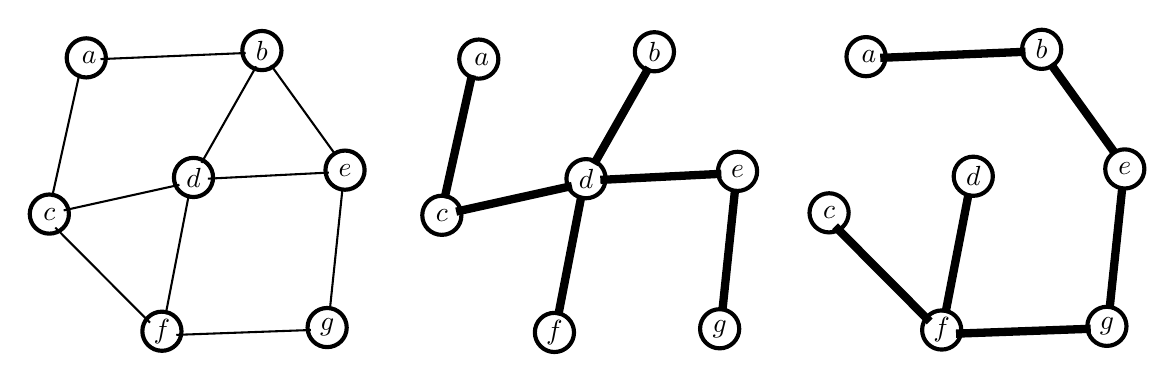
\begin{tikzpicture}[x=0.5pt,y=0.5pt,yscale=-1,xscale=1]
%uncomment if require: \path (0,290); %set diagram left start at 0, and has height of 290

%Straight Lines [id:da6859712806144006] 
\draw [color={rgb, 255:red, 0; green, 0; blue, 0 }  ,draw opacity=1 ][line width=0.75]    (185,39.17) -- (231.39,103.54) ;
%Straight Lines [id:da43828905709564314] 
\draw [color={rgb, 255:red, 0; green, 0; blue, 0 }  ,draw opacity=1 ][line width=0.75]    (116.55,234.06) -- (213.9,230.54) ;
%Straight Lines [id:da6385368954330931] 
\draw [color={rgb, 255:red, 0; green, 0; blue, 0 }  ,draw opacity=1 ][line width=0.75]    (29.1,156.46) -- (97.54,225.24) ;
%Straight Lines [id:da061278223687582845] 
\draw [color={rgb, 255:red, 0; green, 0; blue, 0 }  ,draw opacity=1 ][line width=0.75]    (35.18,144.11) -- (118.84,125.59) ;
%Straight Lines [id:da125058897644165] 
\draw [color={rgb, 255:red, 0; green, 0; blue, 0 }  ,draw opacity=1 ][line width=0.75]    (46.59,45.34) -- (26.81,134.41) ;
%Straight Lines [id:da7561477389708726] 
\draw [color={rgb, 255:red, 0; green, 0; blue, 0 }  ,draw opacity=1 ][line width=0.75]    (61.8,34.76) -- (166.75,30.35) ;
%Straight Lines [id:da8045438090716241] 
\draw [color={rgb, 255:red, 0; green, 0; blue, 0 }  ,draw opacity=1 ][line width=0.75]    (174.35,40.05) -- (134.81,109.72) ;
%Straight Lines [id:da7384444755679203] 
\draw [color={rgb, 255:red, 0; green, 0; blue, 0 }  ,draw opacity=1 ][line width=0.75]    (125.68,132.65) -- (108.95,219.07) ;
%Straight Lines [id:da7781378597799559] 
\draw [color={rgb, 255:red, 0; green, 0; blue, 0 }  ,draw opacity=1 ][line width=0.75]    (236.71,128.24) -- (227.59,215.54) ;
%Straight Lines [id:da6283012441188964] 
\draw [color={rgb, 255:red, 0; green, 0; blue, 0 }  ,draw opacity=1 ][line width=0.75]    (226.83,116.77) -- (139.37,121.18) ;
%Straight Lines [id:da438892015392218] 
\draw [color={rgb, 255:red, 0; green, 0; blue, 0 }  ,draw opacity=1 ][line width=3]    (318.85,144.99) -- (402.51,126.47) ;
%Straight Lines [id:da8359945945218459] 
\draw [color={rgb, 255:red, 0; green, 0; blue, 0 }  ,draw opacity=1 ][line width=3]    (330.26,46.22) -- (310.48,135.29) ;
%Straight Lines [id:da21420370300632352] 
\draw [color={rgb, 255:red, 0; green, 0; blue, 0 }  ,draw opacity=1 ][line width=3]    (458.02,40.93) -- (418.48,110.6) ;
%Straight Lines [id:da9239671202801586] 
\draw [color={rgb, 255:red, 0; green, 0; blue, 0 }  ,draw opacity=1 ][line width=3]    (409.35,133.53) -- (392.62,219.95) ;
%Straight Lines [id:da821215549767216] 
\draw [color={rgb, 255:red, 0; green, 0; blue, 0 }  ,draw opacity=1 ][line width=3]    (520.38,129.12) -- (511.26,216.43) ;
%Straight Lines [id:da9218980242104106] 
\draw [color={rgb, 255:red, 0; green, 0; blue, 0 }  ,draw opacity=1 ][line width=3]    (510.5,117.65) -- (423.04,122.06) ;
%Straight Lines [id:da35247521934474646] 
\draw [color={rgb, 255:red, 0; green, 0; blue, 0 }  ,draw opacity=1 ][line width=3]    (748.54,38.28) -- (794.93,102.66) ;
%Straight Lines [id:da7944029026500893] 
\draw [color={rgb, 255:red, 0; green, 0; blue, 0 }  ,draw opacity=1 ][line width=3]    (680.09,233.18) -- (777.44,229.65) ;
%Straight Lines [id:da39283588857656926] 
\draw [color={rgb, 255:red, 0; green, 0; blue, 0 }  ,draw opacity=1 ][line width=3]    (592.63,155.57) -- (661.08,224.36) ;
%Straight Lines [id:da24731320696047454] 
\draw [color={rgb, 255:red, 0; green, 0; blue, 0 }  ,draw opacity=1 ][line width=3]    (625.33,33.87) -- (730.28,29.46) ;
%Straight Lines [id:da24545478407911292] 
\draw [color={rgb, 255:red, 0; green, 0; blue, 0 }  ,draw opacity=1 ][line width=3]    (689.22,131.76) -- (672.49,218.19) ;
%Straight Lines [id:da379919078999982] 
\draw [color={rgb, 255:red, 0; green, 0; blue, 0 }  ,draw opacity=1 ][line width=3]    (800.25,127.35) -- (791.12,214.66) ;

% Text Node
\draw  [line width=1.5]   (238.52, 115.01) circle [x radius= 14.15, y radius= 14.15]   ;
\draw (238.52,115.01) node   [align=left] {$\displaystyle e$};
% Text Node
\draw  [line width=1.5]   (51.52, 33.87) circle [x radius= 14.15, y radius= 14.15]   ;
\draw (46.02,33.87) node [anchor=west] [inner sep=0.75pt]   [align=left] {$\displaystyle a$};
% Text Node
\draw  [line width=1.5]   (178.44, 28.58) circle [x radius= 14.15, y radius= 14.15]   ;
\draw (178.44,28.58) node   [align=left] {$\displaystyle b$};
% Text Node
\draw  [line width=1.5]   (24.82, 146.76) circle [x radius= 14.15, y radius= 14.15]   ;
\draw (24.82,146.76) node   [align=left] {$\displaystyle c$};
% Text Node
\draw  [line width=1.5]   (129.01, 120.3) circle [x radius= 14.15, y radius= 14.15]   ;
\draw (129.01,120.3) node   [align=left] {$\displaystyle d$};
% Text Node
\draw  [line width=1.5]   (106.19, 231.42) circle [x radius= 14.15, y radius= 14.15]   ;
\draw (106.19,231.42) node   [align=left] {$\displaystyle f$};
% Text Node
\draw  [line width=1.5]   (225.59, 228.77) circle [x radius= 14.15, y radius= 14.15]   ;
\draw (225.59,228.77) node   [align=left] {$\displaystyle g$};
% Text Node
\draw  [line width=1.5]   (522.19, 115.89) circle [x radius= 14.15, y radius= 14.15]   ;
\draw (522.19,115.89) node   [align=left] {$\displaystyle e$};
% Text Node
\draw  [line width=1.5]   (335.19, 34.76) circle [x radius= 14.15, y radius= 14.15]   ;
\draw (329.69,34.76) node [anchor=west] [inner sep=0.75pt]   [align=left] {$\displaystyle a$};
% Text Node
\draw  [line width=1.5]   (462.11, 29.46) circle [x radius= 14.15, y radius= 14.15]   ;
\draw (462.11,29.46) node   [align=left] {$\displaystyle b$};
% Text Node
\draw  [line width=1.5]   (308.49, 147.64) circle [x radius= 14.15, y radius= 14.15]   ;
\draw (308.49,147.64) node   [align=left] {$\displaystyle c$};
% Text Node
\draw  [line width=1.5]   (412.68, 121.18) circle [x radius= 14.15, y radius= 14.15]   ;
\draw (412.68,121.18) node   [align=left] {$\displaystyle d$};
% Text Node
\draw  [line width=1.5]   (389.86, 232.3) circle [x radius= 14.15, y radius= 14.15]   ;
\draw (389.86,232.3) node   [align=left] {$\displaystyle f$};
% Text Node
\draw  [line width=1.5]   (509.26, 229.65) circle [x radius= 14.15, y radius= 14.15]   ;
\draw (509.26,229.65) node   [align=left] {$\displaystyle g$};
% Text Node
\draw  [line width=1.5]   (802.06, 114.13) circle [x radius= 14.15, y radius= 14.15]   ;
\draw (802.06,114.13) node   [align=left] {$\displaystyle e$};
% Text Node
\draw  [line width=1.5]   (615.06, 32.99) circle [x radius= 14.15, y radius= 14.15]   ;
\draw (609.56,32.99) node [anchor=west] [inner sep=0.75pt]   [align=left] {$\displaystyle a$};
% Text Node
\draw  [line width=1.5]   (741.98, 27.7) circle [x radius= 14.15, y radius= 14.15]   ;
\draw (741.98,27.7) node   [align=left] {$\displaystyle b$};
% Text Node
\draw  [line width=1.5]   (588.35, 145.87) circle [x radius= 14.15, y radius= 14.15]   ;
\draw (588.35,145.87) node   [align=left] {$\displaystyle c$};
% Text Node
\draw  [line width=1.5]   (692.54, 119.42) circle [x radius= 14.15, y radius= 14.15]   ;
\draw (692.54,119.42) node   [align=left] {$\displaystyle d$};
% Text Node
\draw  [line width=1.5]   (669.73, 230.54) circle [x radius= 14.15, y radius= 14.15]   ;
\draw (669.73,230.54) node   [align=left] {$\displaystyle f$};
% Text Node
\draw  [line width=1.5]   (789.13, 227.89) circle [x radius= 14.15, y radius= 14.15]   ;
\draw (789.13,227.89) node   [align=left] {$\displaystyle g$};


\end{tikzpicture}

